\documentclass[pdflatex,compress,mathserif]{beamer}

%\usetheme[dark,framenumber,totalframenumber]{ElektroITK}
\usetheme[darktitle,framenumber,totalframenumber]{ElektroITK}

\usepackage[utf8]{inputenc}
\usepackage[T1]{fontenc}
\usepackage{lmodern}
\usepackage[bahasai]{babel}
\usepackage{amsmath}
\usepackage{amsfonts}
\usepackage{amssymb}
\usepackage{graphicx}
\usepackage{multicol}
\usepackage{lipsum}
\usepackage{media9}
\usefonttheme[onlymath]{serif}

\newcommand*{\Scale}[2][4]{\scalebox{#1}{$#2$}}%

\renewcommand\thempfootnote{\arabic{mpfootnote}} % footnote arabic number

\setbeamertemplate{caption}[numbered]

\title{KECERDASAN BUATAN}
\subtitle{FUZZY LOGIC}

\author{Mifta Nur Farid}
\date{15 Februari 2024}

\begin{document}

\maketitle

\begin{frame}{Pengantar}
	\begin{center}
		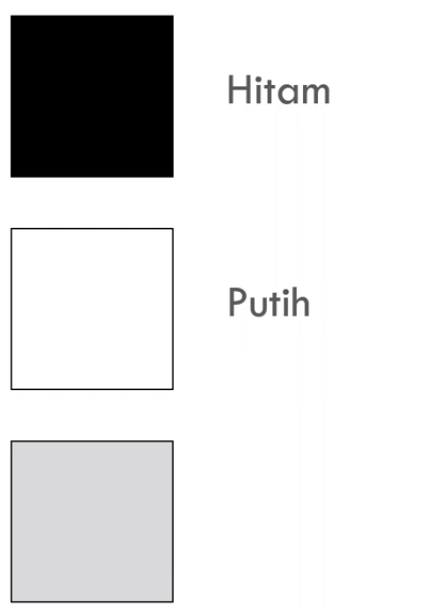
\includegraphics[height=0.7\textheight]{img/01}
	\end{center}
\end{frame}

\begin{frame}{Pengantar}
	\begin{center}
		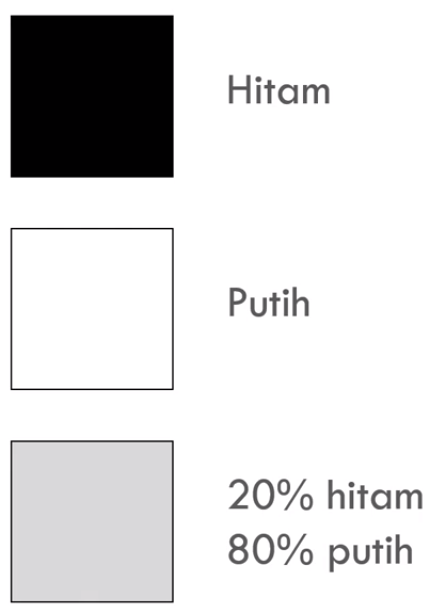
\includegraphics[height=0.7\textheight]{img/02}
	\end{center}
\end{frame}

\begin{frame}{Pengantar}
	\begin{center}
		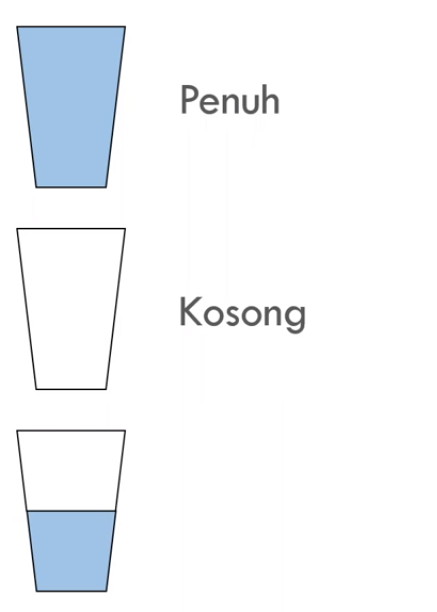
\includegraphics[height=0.7\textheight]{img/03}
	\end{center}
\end{frame}

\begin{frame}{Pengantar}
	\begin{center}
		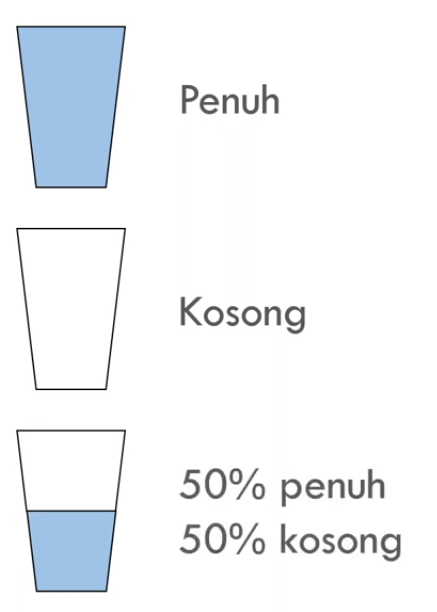
\includegraphics[height=0.7\textheight]{img/04}
	\end{center}
\end{frame}

\begin{frame}{Pengantar}
	\begin{center}
		\Large{APA KAITANNYA DENGAN FUZZY LOGIC?}
	\end{center}
\end{frame}

\begin{frame}{Pengantar}
	\begin{itemize}
		\item Ada hal-hal yang tidak bisa dipandang sebagai HITAM DAN PUTIH maupun TRUE DAN FALSE
		\item Karena ada sesuatu yang bernilai diantara keduanya
		\item Fuzzy Logic memberikan solusi.
	\end{itemize}
\end{frame}

\begin{frame}{Fuzzy Logic}
	\begin{itemize}
		\item Logika yang memiliki nilai kebenaran dari 0 hingga 1
		\item Logika yang yang tidak hanya bernilai TRUE dan FALSE
		\item Kegunaan:
		\begin{enumerate}
			\item Decision support
			\item System control
			\item Prediction
		\end{enumerate}
	\end{itemize}
\end{frame}

\begin{frame}{Nilai Kebenaran}
	\begin{itemize}
		\item Nilai yang menyatakan kecenderungan terhadap suatu kelompok nilai
		\begin{center}
			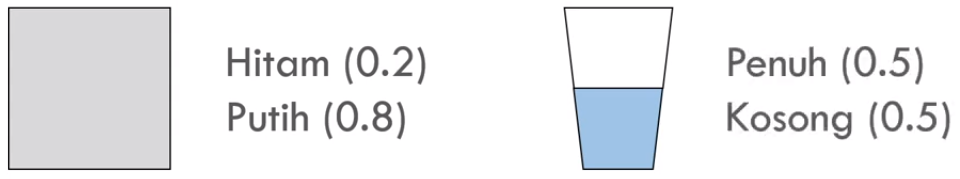
\includegraphics[width=0.6\linewidth]{img/05}
		\end{center}
		\item Nilai kebenaran = Nilai keanggotaan
	\end{itemize}
\end{frame}

\begin{frame}{Fungsi Keanggotaan}
	\begin{itemize}
		\item Fungsi matematika untuk menentukan nilai keanggotaan
		\begin{center}
			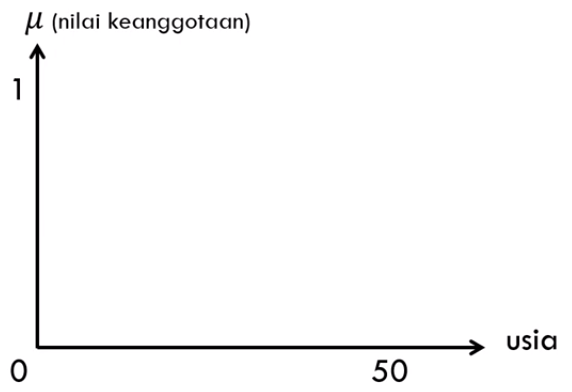
\includegraphics[width=0.5\linewidth]{img/06}
		\end{center}
	\end{itemize}
\end{frame}

\begin{frame}{Fungsi Keanggotaan}
	\begin{itemize}
		\item Fungsi matematika untuk menentukan nilai keanggotaan
		\begin{center}
			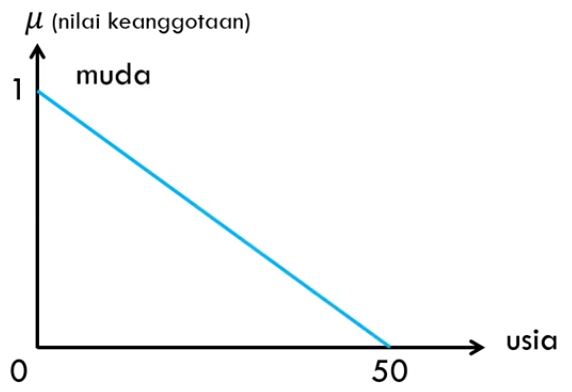
\includegraphics[width=0.5\linewidth]{img/07}
		\end{center}
	\end{itemize}
\end{frame}

\begin{frame}{Fungsi Keanggotaan}
	\begin{itemize}
		\item Fungsi matematika untuk menentukan nilai keanggotaan
		\begin{center}
			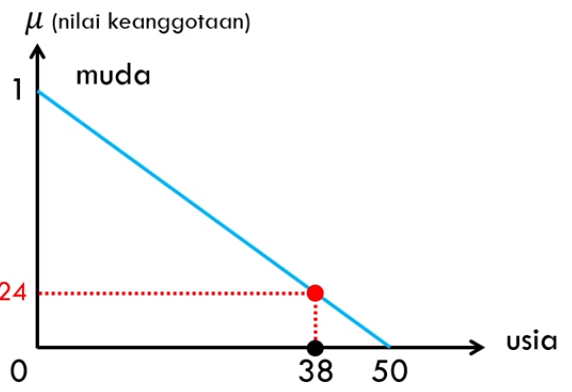
\includegraphics[width=0.5\linewidth]{img/08}
		\end{center}
	\end{itemize}
\end{frame}

\begin{frame}{Fungsi Keanggotaan}
	\begin{itemize}
		\item Fungsi matematika untuk menentukan nilai keanggotaan
		\begin{multicols}{2}
			\begin{center}
				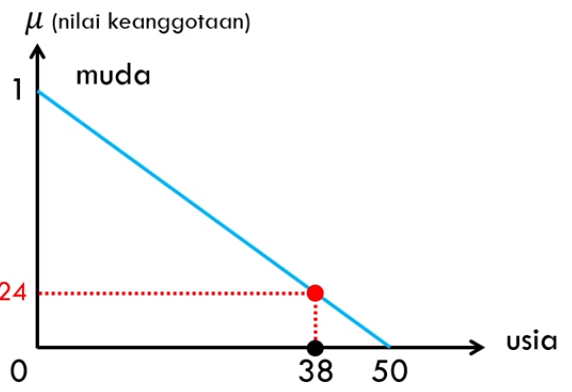
\includegraphics[width=\linewidth]{img/08}
			\end{center}
			\columnbreak
			\begin{align*}
				\mu_{\text{muda}}(38) &= \frac{50 - 38}{50 - 0} \\
				&= 0.24 \\
				&= \text{\textbf{Muda(0.24)}}
			\end{align*}
		\end{multicols}
	\end{itemize}
\end{frame}

\begin{frame}{Fungsi Keanggotaan}
	\begin{itemize}
		\item Fungsi matematika untuk menentukan nilai keanggotaan
		\begin{center}
			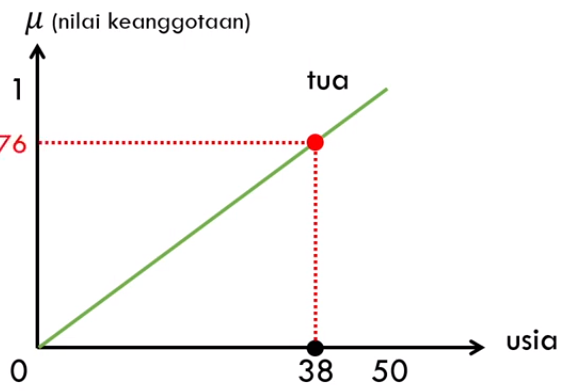
\includegraphics[width=0.5\linewidth]{img/09}
		\end{center}
	\end{itemize}
\end{frame}

\begin{frame}{Fungsi Keanggotaan}
	\begin{itemize}
		\item Fungsi matematika untuk menentukan nilai keanggotaan
		\begin{multicols}{2}
			\begin{center}
				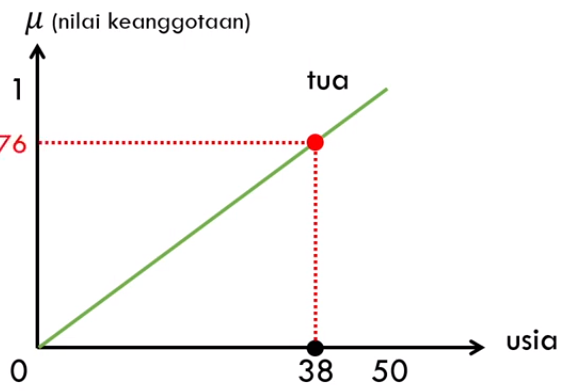
\includegraphics[width=\linewidth]{img/09}
			\end{center}
			\columnbreak
			\begin{align*}
				\mu_{\text{tua}}(38) &= \frac{38 - 0}{50 - 0} \\
				&= 0.76 \\
				&= \text{\textbf{Tua(0.76)}}
			\end{align*}
		\end{multicols}
	\end{itemize}
\end{frame}

\begin{frame}{Fungsi Keanggotaan}
	\begin{itemize}
		\item Fungsi matematika untuk menentukan nilai keanggotaan
		\begin{center}
			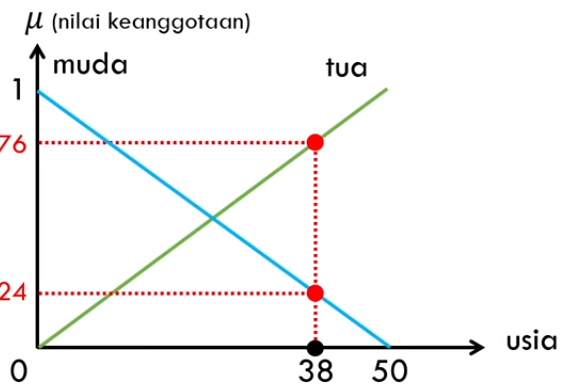
\includegraphics[width=0.5\linewidth]{img/10}
		\end{center}
	\end{itemize}
\end{frame}

\begin{frame}{Fungsi Keanggotaan}
	\begin{itemize}
		\item Fungsi matematika untuk menentukan nilai keanggotaan
		\begin{multicols}{2}
			\begin{center}
				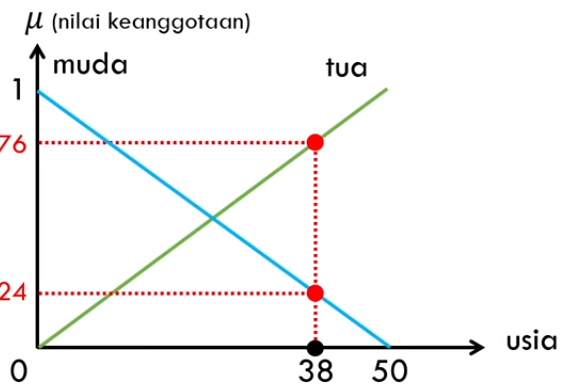
\includegraphics[width=\linewidth]{img/10}
			\end{center}
			\columnbreak
			\begin{align*}
				\mu_{\text{muda}}(38) &= \text{\textbf{Muda(0.24)}} \\
				\mu_{\text{tua}}(38) &= \text{\textbf{Tua(0.76)}} 
			\end{align*}
		\end{multicols}
	\end{itemize}
\end{frame}

\begin{frame}{Fungsi Keanggotaan}
	\begin{itemize}
		\item Fungsi matematika untuk menentukan nilai keanggotaan
		\begin{center}
			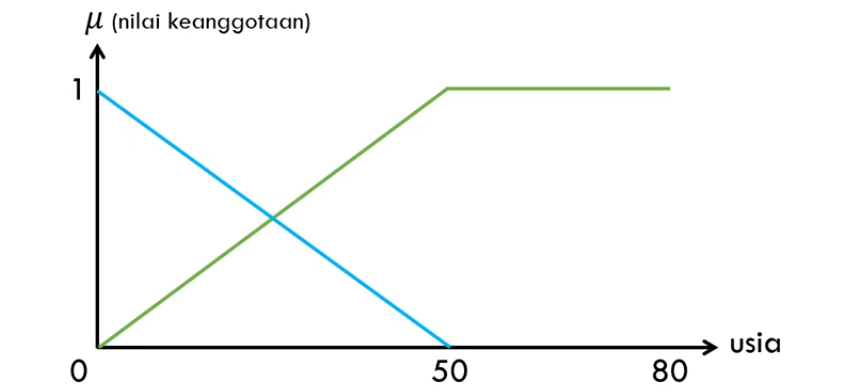
\includegraphics[width=0.7\linewidth]{img/12}
		\end{center}
	\end{itemize}
\end{frame}

\begin{frame}{Fungsi Keanggotaan}
	\begin{itemize}
		\item Fungsi matematika untuk menentukan nilai keanggotaan
		\begin{center}
			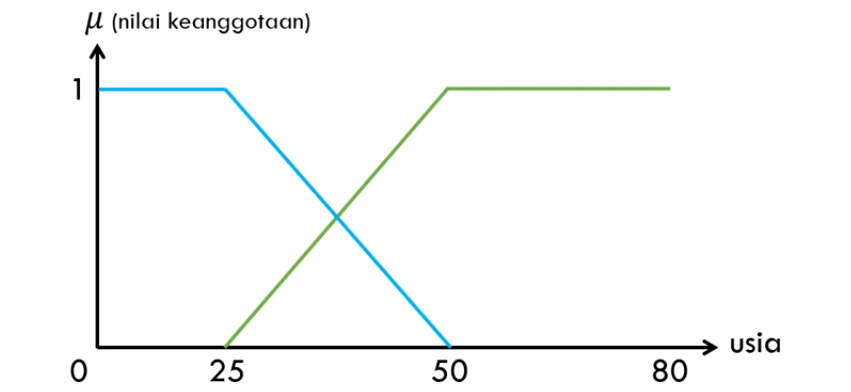
\includegraphics[width=0.7\linewidth]{img/11}
		\end{center}
	\end{itemize}
\end{frame}

\begin{frame}{Fungsi Keanggotaan}
	\begin{itemize}
		\item Fungsi matematika untuk menentukan nilai keanggotaan
		\begin{center}
			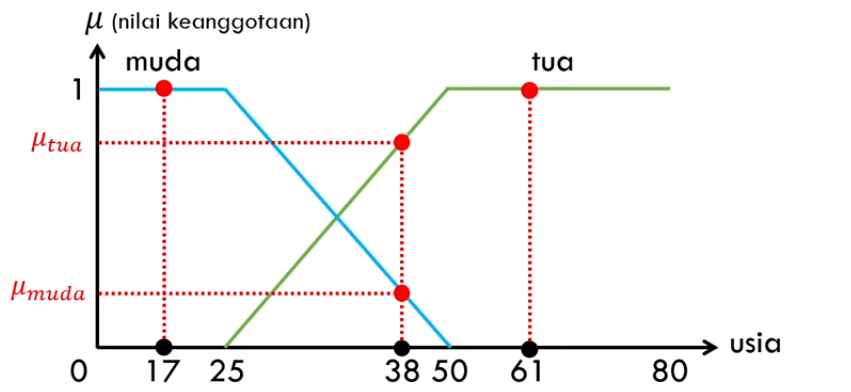
\includegraphics[width=0.7\linewidth]{img/13}
		\end{center}
	\end{itemize}
\end{frame}

\begin{frame}{Fungsi Keanggotaan}
	\begin{itemize}
		\item Fungsi Linear Turun
		\begin{center}
			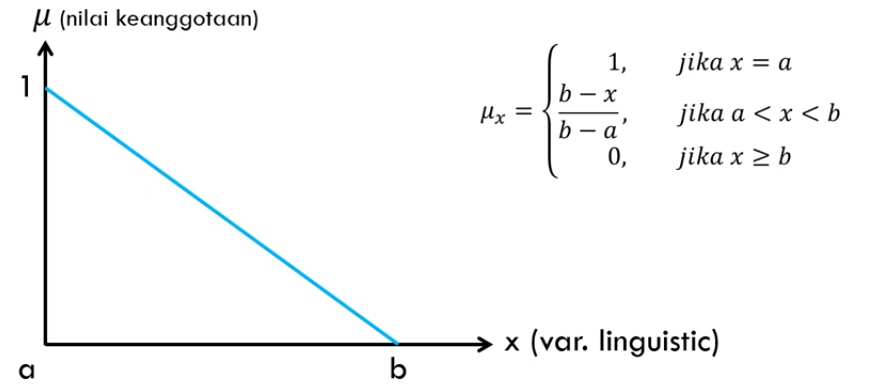
\includegraphics[width=\linewidth]{img/14}
		\end{center}
	\end{itemize}
 \end{frame}

\begin{frame}{Fungsi Keanggotaan}
	\begin{itemize}
		\item Fungsi Linear Naik
		\begin{center}
			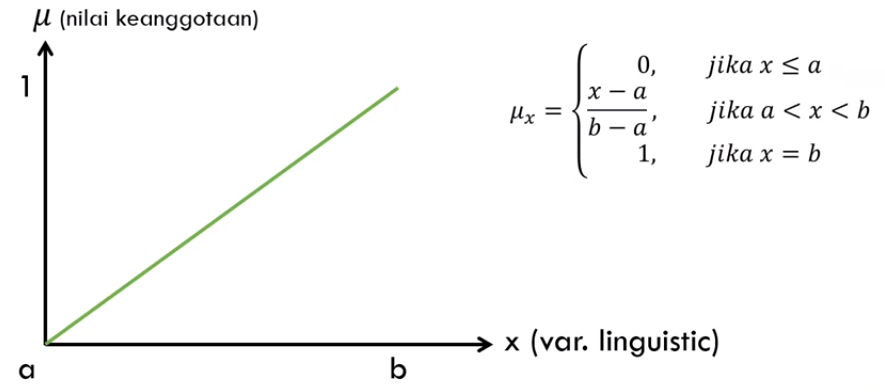
\includegraphics[width=\linewidth]{img/15}
		\end{center}
	\end{itemize}
\end{frame}

\begin{frame}{Fungsi Keanggotaan}
	\begin{itemize}
		\item Fungsi Segitiga
		\begin{center}
			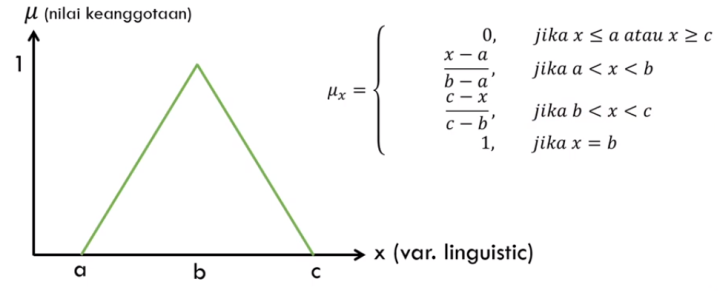
\includegraphics[width=\linewidth]{img/16}
		\end{center}
	\end{itemize}
\end{frame}

\begin{frame}{Fungsi Keanggotaan}
	\begin{itemize}
		\item Fungsi Trapesium
		\begin{center}
			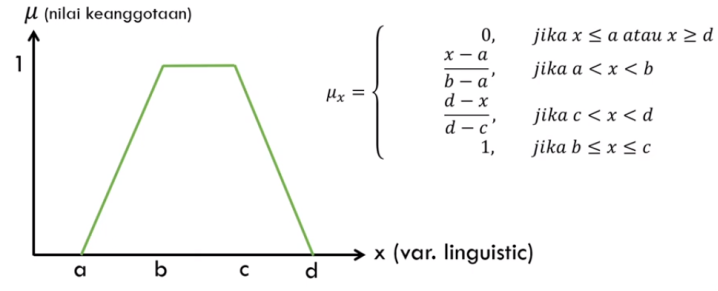
\includegraphics[width=\linewidth]{img/17}
		\end{center}
	\end{itemize}
\end{frame}

\begin{frame}{Fungsi Keanggotaan}
	\begin{center}
		Masih ada beberapa bentuk fungsi keanggotaan yang lain. Silakan dipelajari sendiri.
	\end{center}
\end{frame}

\begin{frame}{Fungsi Keanggotaan}
	\begin{itemize}
		\item Variabel linguistik: Usia
		\item Nilai linguistik: muda, paruh baya, tua
	\end{itemize}
	\begin{center}
		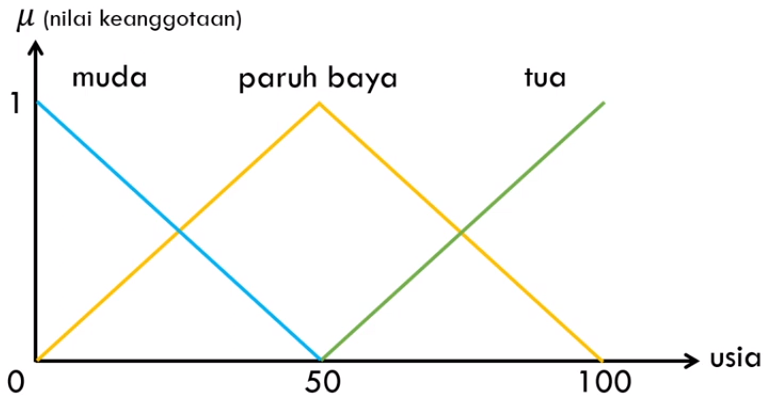
\includegraphics[width=0.7\linewidth]{img/18}
	\end{center}
\end{frame}

\begin{frame}{Fungsi Keanggotaan}
	\begin{itemize}
		\item Tidak harus simetris
	\end{itemize}
	\begin{center}
		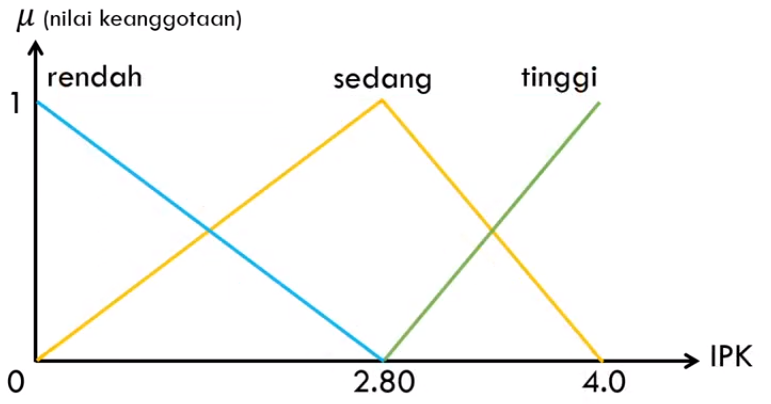
\includegraphics[width=0.7\linewidth]{img/19}
	\end{center}
\end{frame}

\begin{frame}{Fungsi Keanggotaan}
	\begin{itemize}
		\item Perpaduan
	\end{itemize}
	\begin{center}
		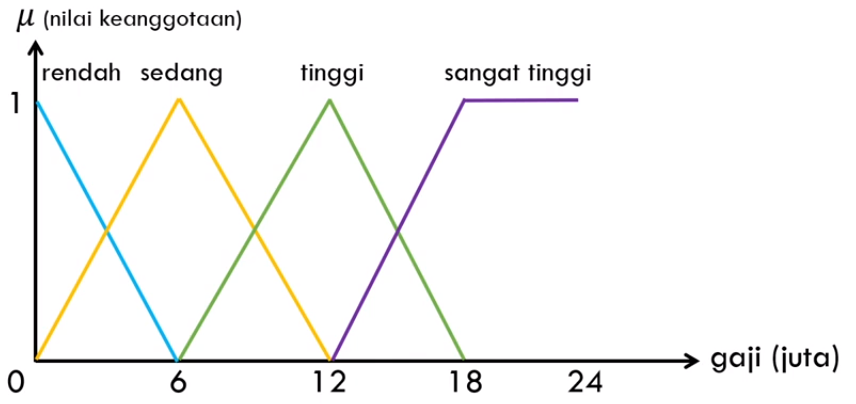
\includegraphics[width=0.7\linewidth]{img/20}
	\end{center}
\end{frame}

\begin{frame}{Fungsi Keanggotaan}
	\begin{itemize}
		\item Perpaduan
	\end{itemize}
	\begin{center}
		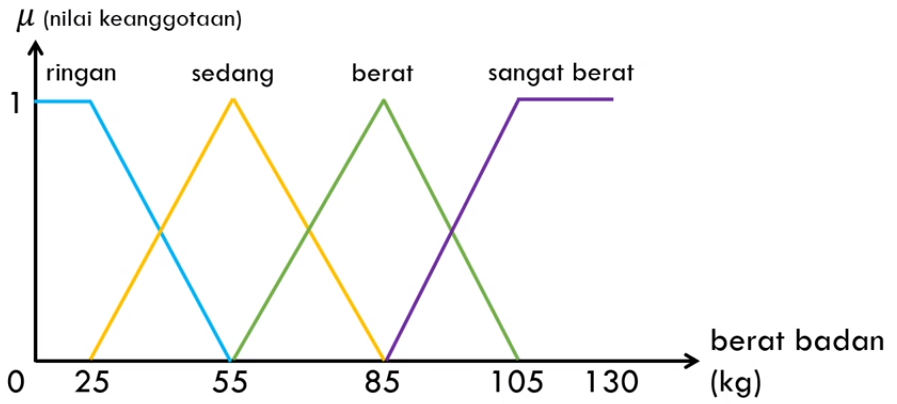
\includegraphics[width=0.7\linewidth]{img/21}
	\end{center}
\end{frame}

\begin{frame}{Studi Kasus}
	\begin{itemize}
		\item Merancang sistem pengaturan \textbf{durasi pencucian} pada mesin cuci berdasarkan \textbf{berat pakaian} dan \textbf{intensitas kotoran}
		\item Misal, berat pakaian \textbf{6.8 kg} dan intensitas kotoran \textbf{45\%}
		\item Bagaimana penyelesaiannya dengan menggunakan Fuzzy Logic?
	\end{itemize}
\end{frame}

\begin{frame}{Fuzzy Logic}
	\begin{center}
		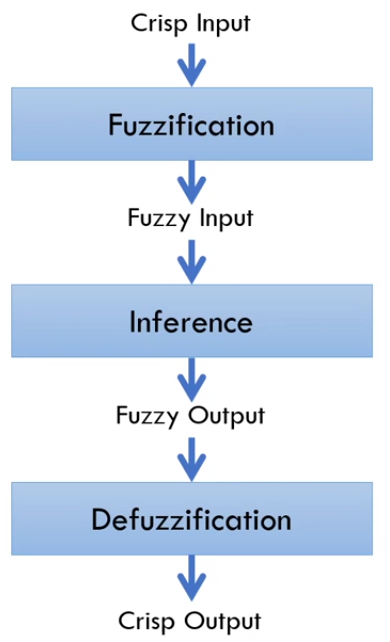
\includegraphics[height=0.8\textheight]{img/22}
	\end{center}
\end{frame}

\begin{frame}{Fuzzification}
	\begin{itemize}
		\item Crisp Input: berat pakaian \textbf{6.8 kg} dan intensitas kotoran \textbf{45\%}
	\end{itemize}
\end{frame}

\begin{frame}{Fuzzification}
	\begin{center}
		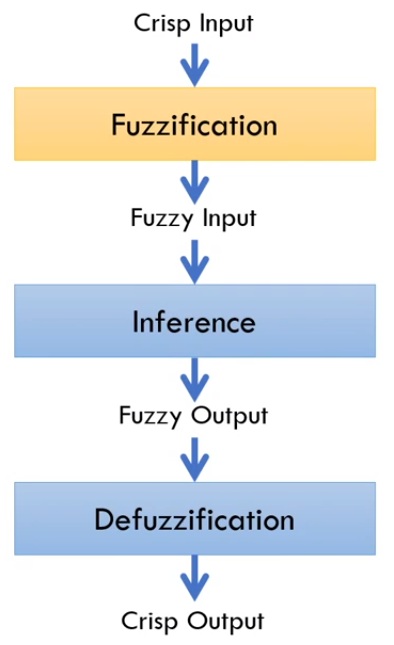
\includegraphics[height=0.8\textheight]{img/fuzzification}
	\end{center}
\end{frame}

\begin{frame}{Fuzzification}
	\begin{center}
		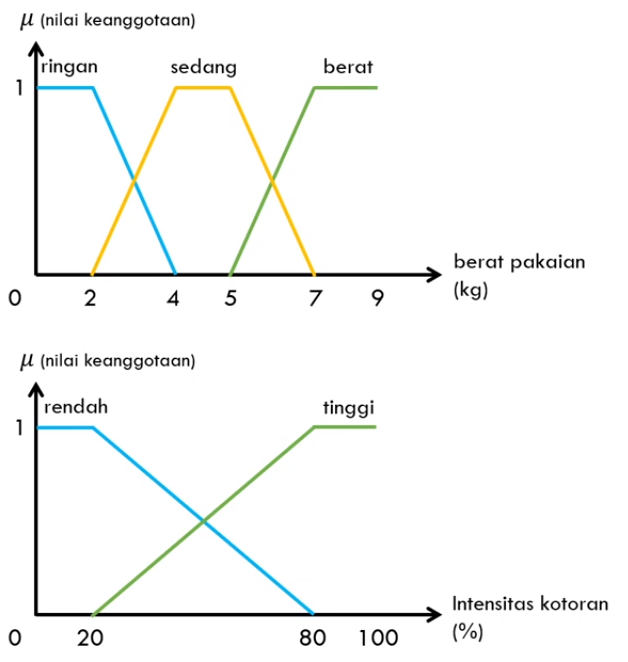
\includegraphics[height=0.9\textheight]{img/23}
	\end{center}
\end{frame}

\begin{frame}{Fuzzification}
	\begin{center}
		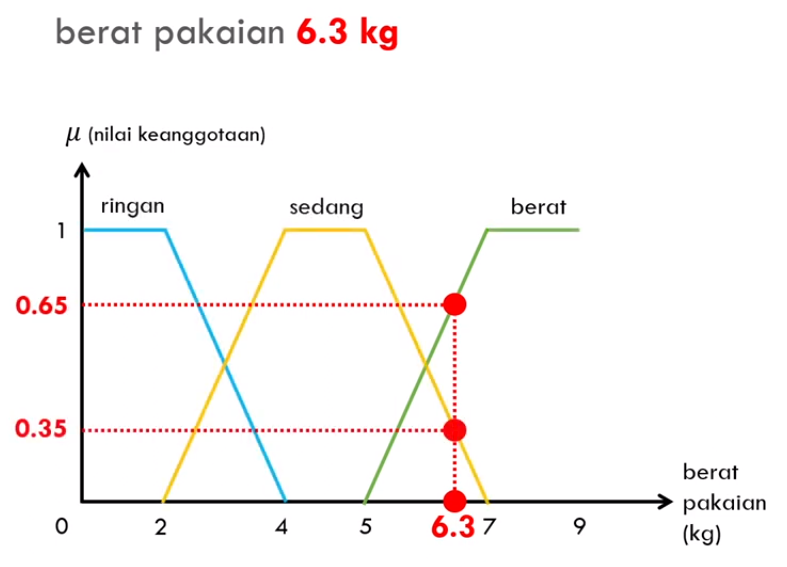
\includegraphics[height=0.8\textheight]{img/24}
	\end{center}
\end{frame}

\begin{frame}{Fuzzification}
	\begin{center}
		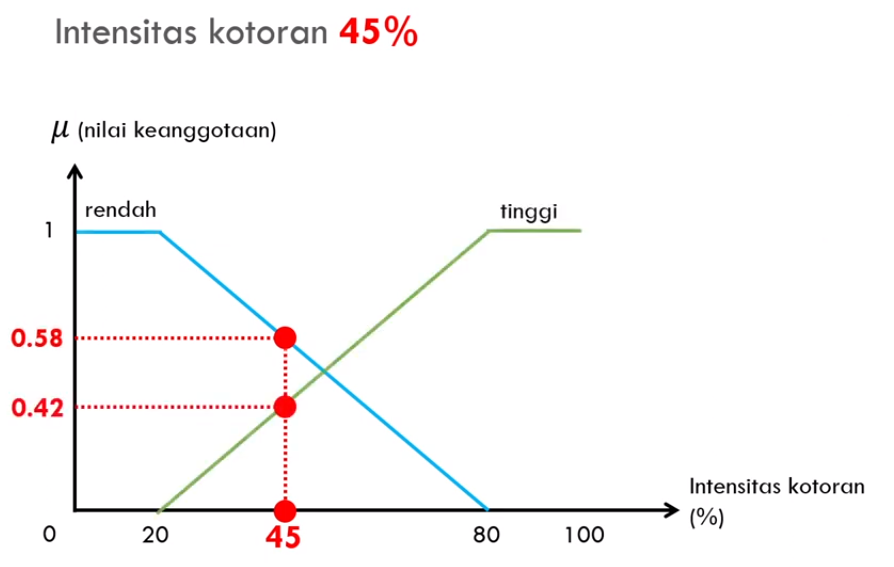
\includegraphics[height=0.8\textheight]{img/25}
	\end{center}
\end{frame}

\begin{frame}{Fuzzification}
	\begin{center}
		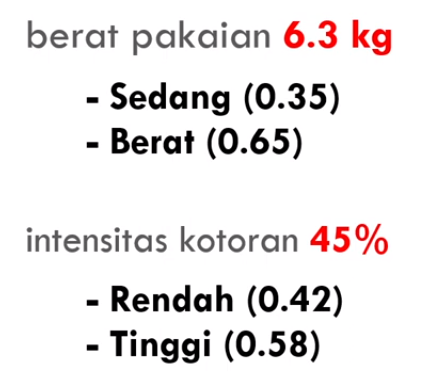
\includegraphics[height=0.6\textheight]{img/26}
	\end{center}
\end{frame}

\begin{frame}{Fuzzification}
	\begin{center}
		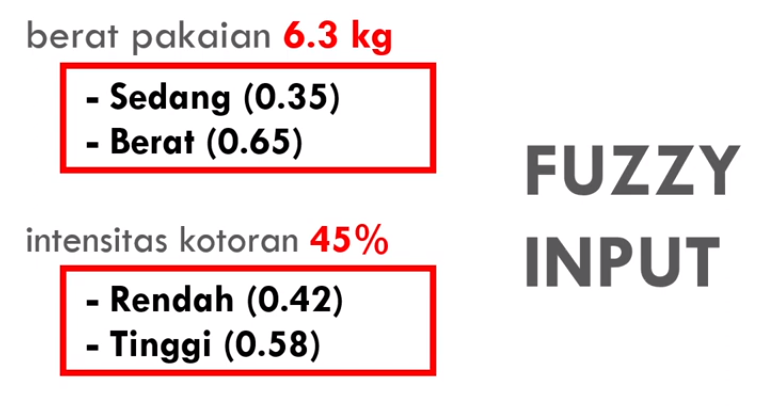
\includegraphics[height=0.6\textheight]{img/27}
	\end{center}
\end{frame}

\begin{frame}{Inference}
	\begin{center}
		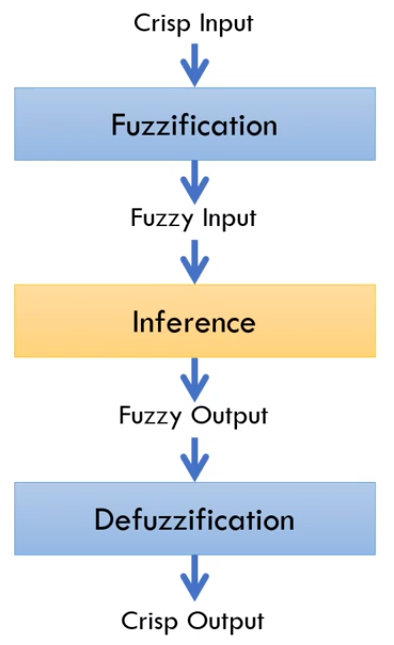
\includegraphics[height=0.8\textheight]{img/inference}
	\end{center}
\end{frame}

\begin{frame}{Inference}
	\begin{center}
		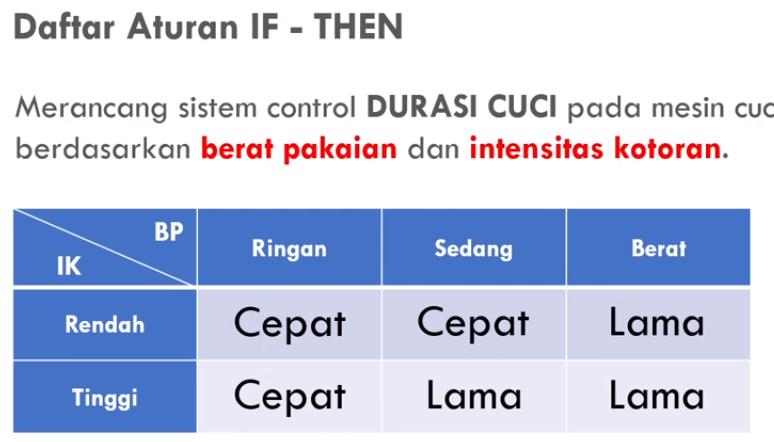
\includegraphics[height=0.6\textheight]{img/28}
	\end{center}
\end{frame}

\begin{frame}{Inference}
	\begin{center}
		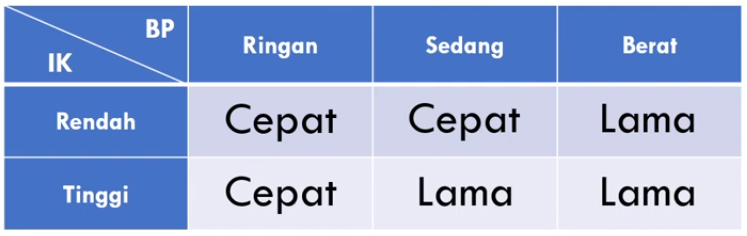
\includegraphics[height=0.3\textheight]{img/29a}
		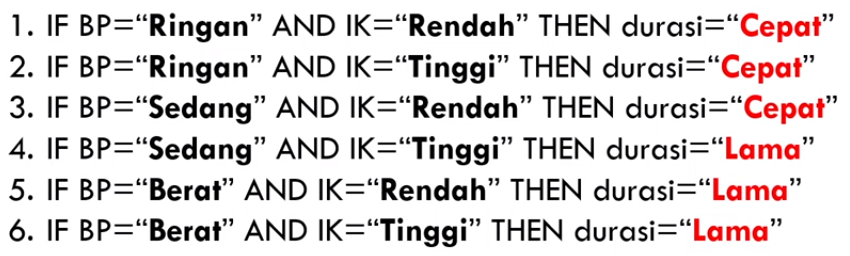
\includegraphics[height=0.4\textheight]{img/29b}
	\end{center}
\end{frame}

\begin{frame}{Inference}
	\begin{center}
		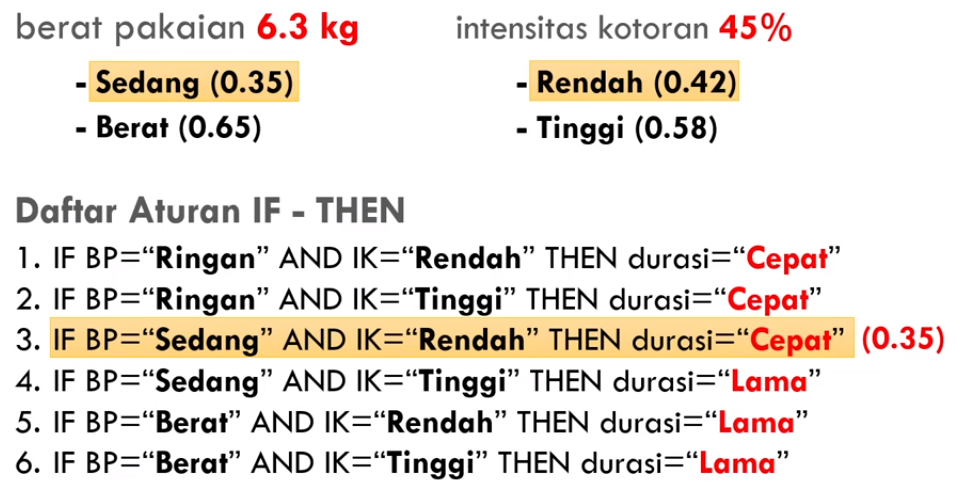
\includegraphics[width=\linewidth]{img/30}
	\end{center}
\end{frame}

\begin{frame}{Inference}
	\begin{center}
		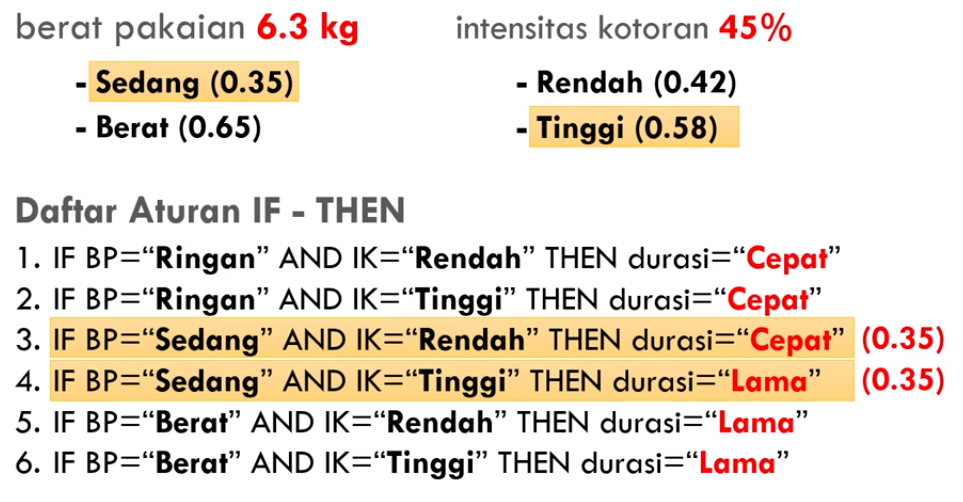
\includegraphics[width=\linewidth]{img/31}
	\end{center}
\end{frame}

\begin{frame}{Inference}
	\begin{center}
		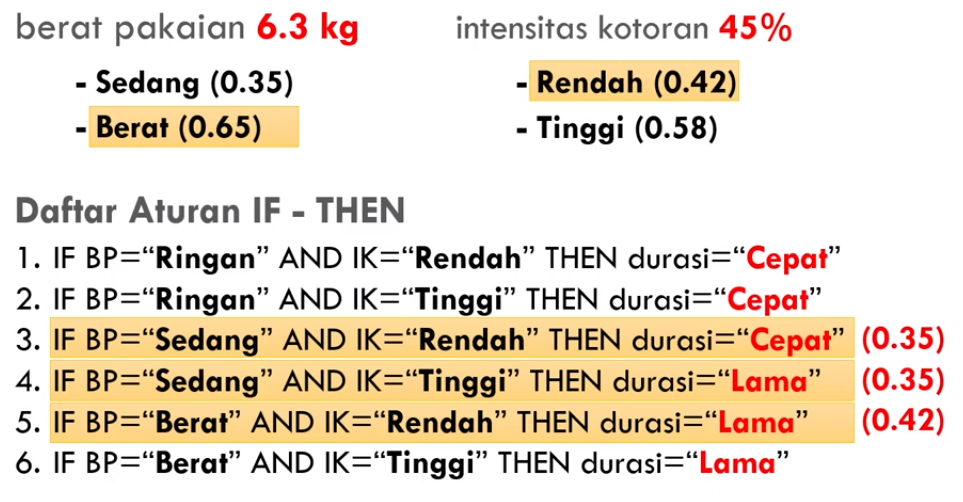
\includegraphics[width=\linewidth]{img/32}
	\end{center}
\end{frame}

\begin{frame}{Inference}
	\begin{center}
		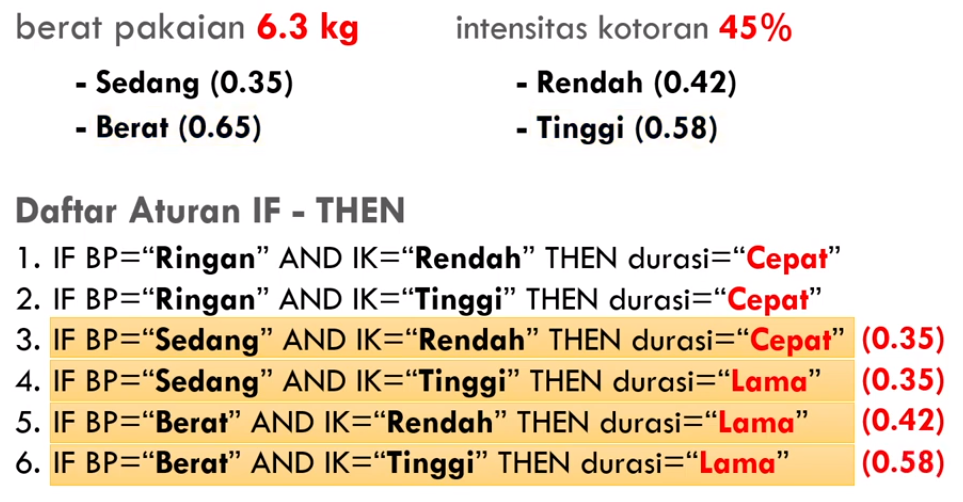
\includegraphics[width=\linewidth]{img/33}
	\end{center}
\end{frame}

\begin{frame}{Inference}
	\begin{center}
		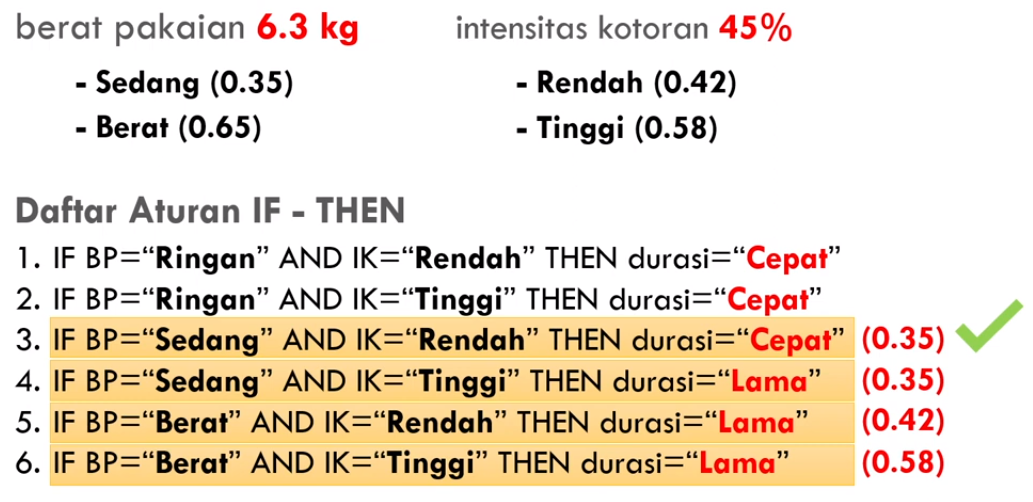
\includegraphics[width=\linewidth]{img/34}
	\end{center}
\end{frame}

\begin{frame}{Inference}
	\begin{center}
		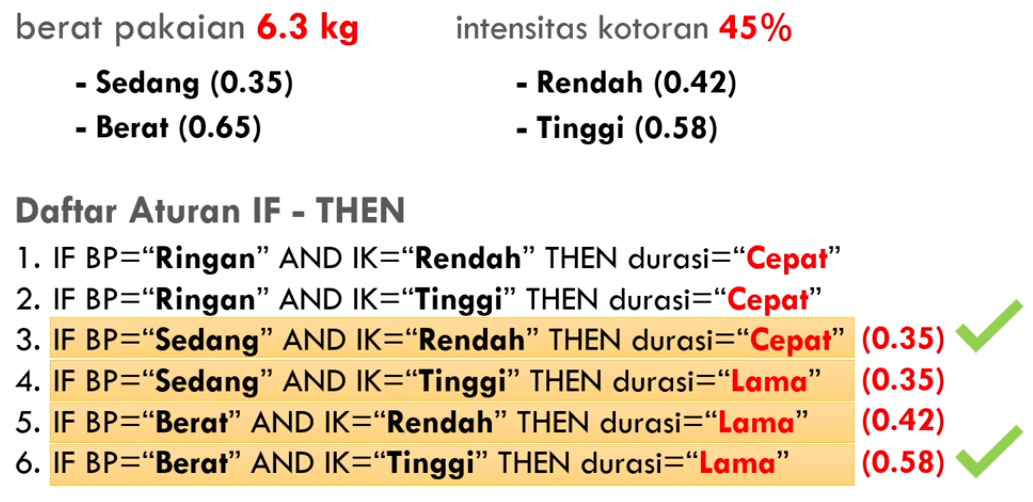
\includegraphics[width=\linewidth]{img/35}
	\end{center}
\end{frame}

\begin{frame}{Inference}
	\begin{center}
		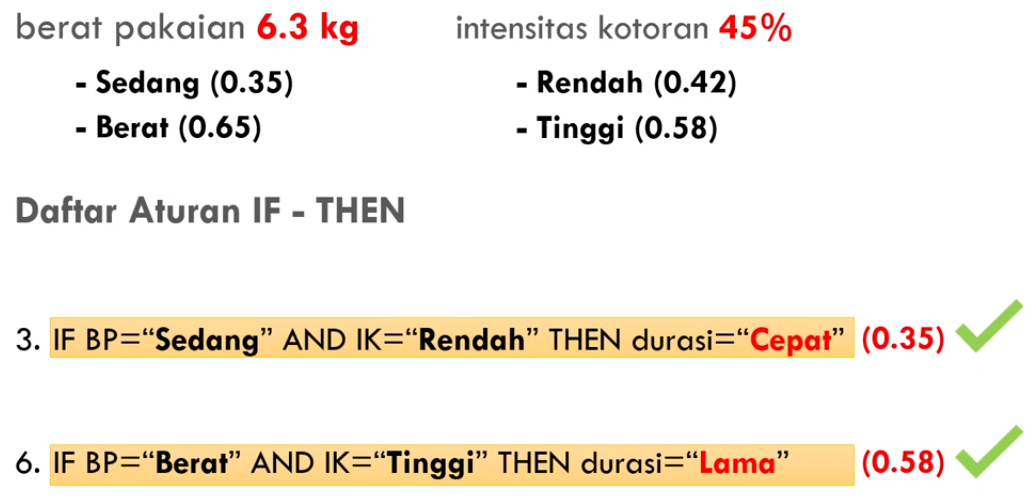
\includegraphics[width=\linewidth]{img/36}
	\end{center}
\end{frame}

\begin{frame}{Inference}
	\begin{center}
		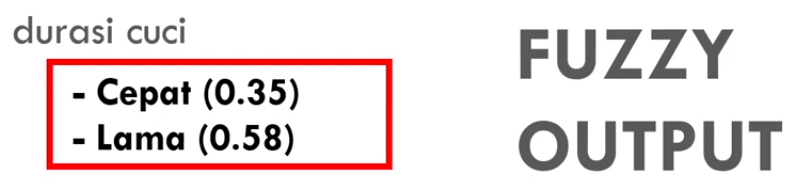
\includegraphics[width=\linewidth]{img/37}
	\end{center}
\end{frame}

\begin{frame}{Defuzification}
	\begin{center}
		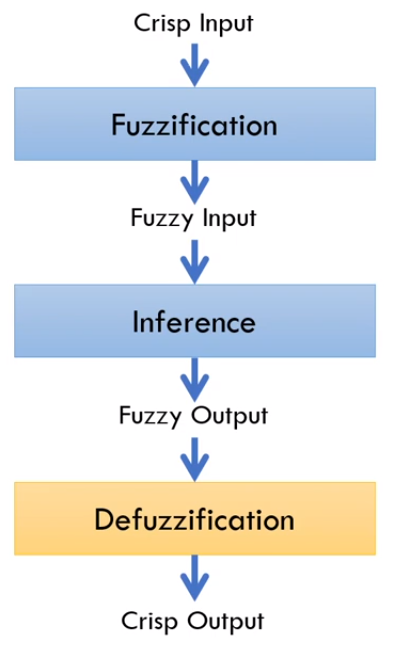
\includegraphics[height=0.8\textheight]{img/defuzzification}
	\end{center}
\end{frame}

\begin{frame}{Defuzification}
	\begin{center}
		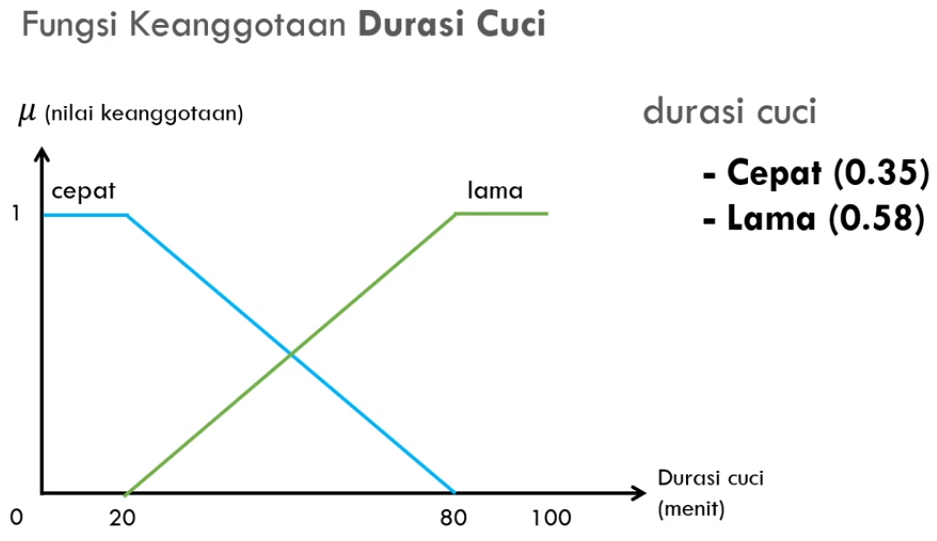
\includegraphics[height=0.8\textheight]{img/38}
	\end{center}
\end{frame}

\begin{frame}{Defuzification}
	\begin{enumerate}
		\item Tsukamoto
		\item Mamdani
		\item Sugeno
	\end{enumerate}
\end{frame}

\begin{frame}{Defuzification - Tsukamoto}
	\begin{center}
		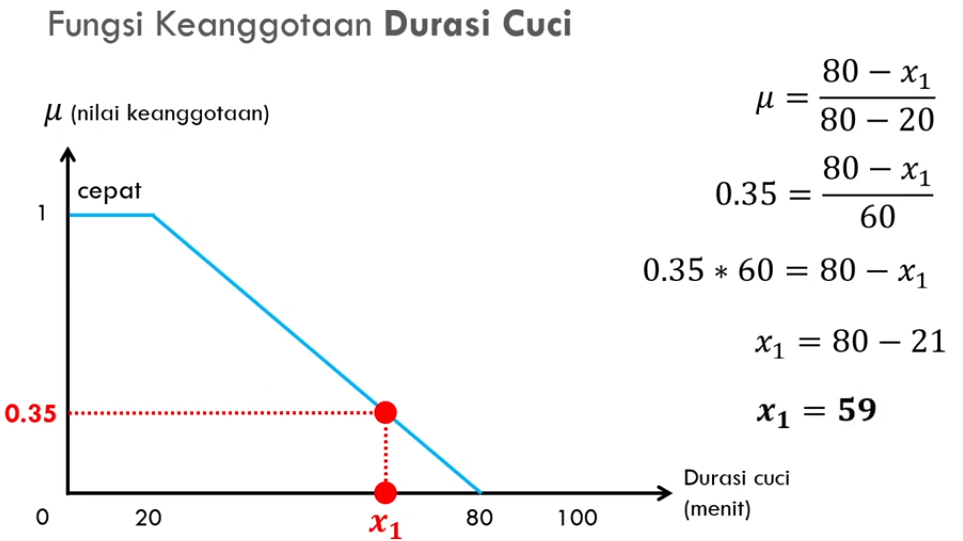
\includegraphics[height=0.8\textheight]{img/39}
	\end{center}
\end{frame}

\begin{frame}{Defuzification - Tsukamoto}
	\begin{center}
		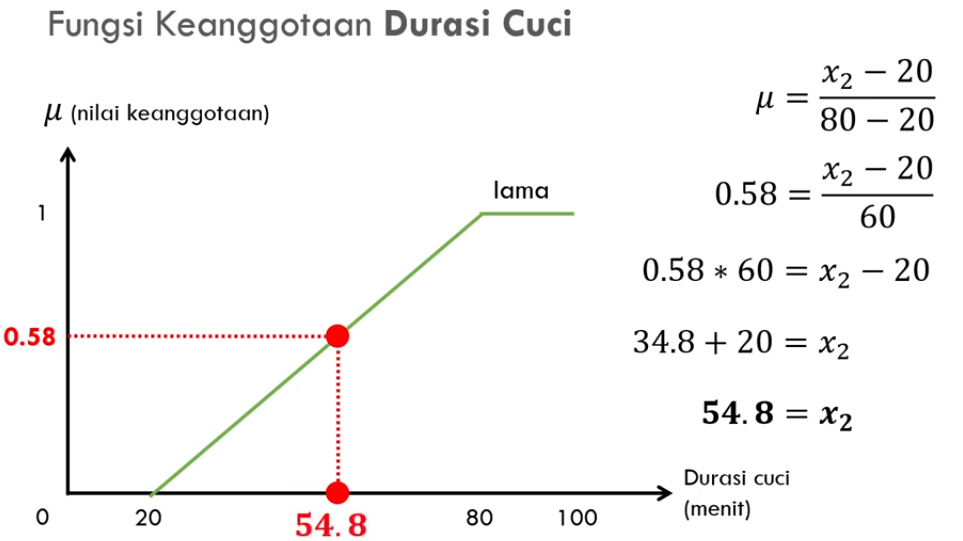
\includegraphics[height=0.8\textheight]{img/40}
	\end{center}
\end{frame}

\begin{frame}{Defuzification - Tsukamoto}
	\begin{center}
		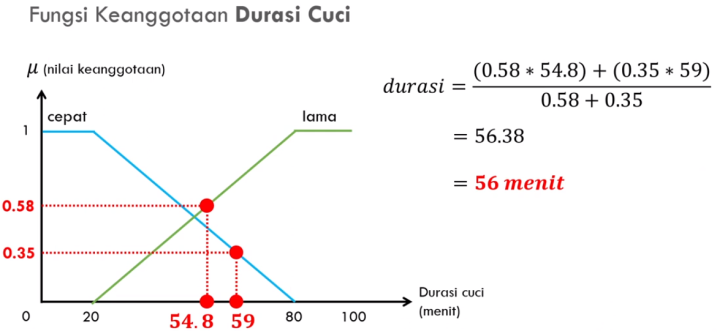
\includegraphics[width=\linewidth]{img/41}
	\end{center}
\end{frame}

\begin{frame}{Defuzification - Mamdani}
	\begin{center}
		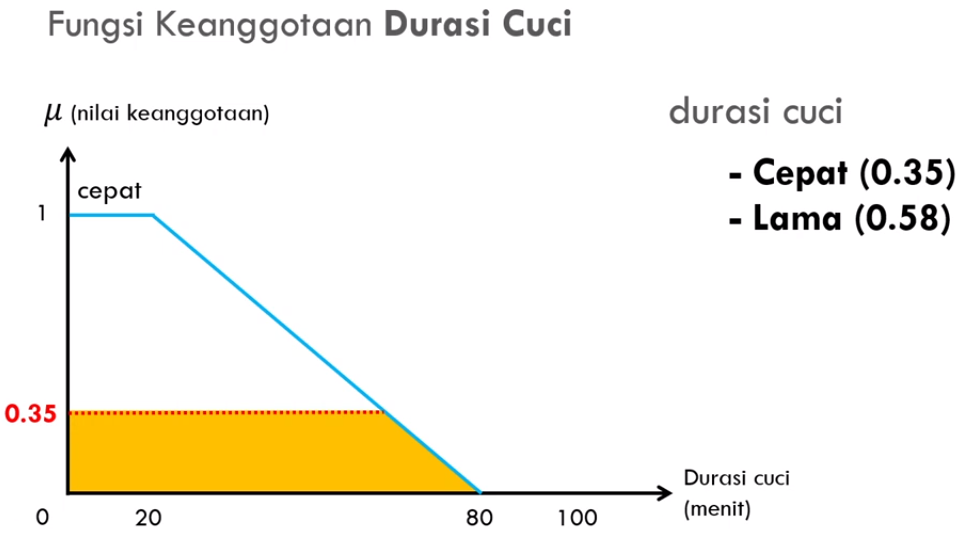
\includegraphics[width=\linewidth]{img/42}
	\end{center}
\end{frame}

\begin{frame}{Defuzification - Mamdani}
	\begin{center}
		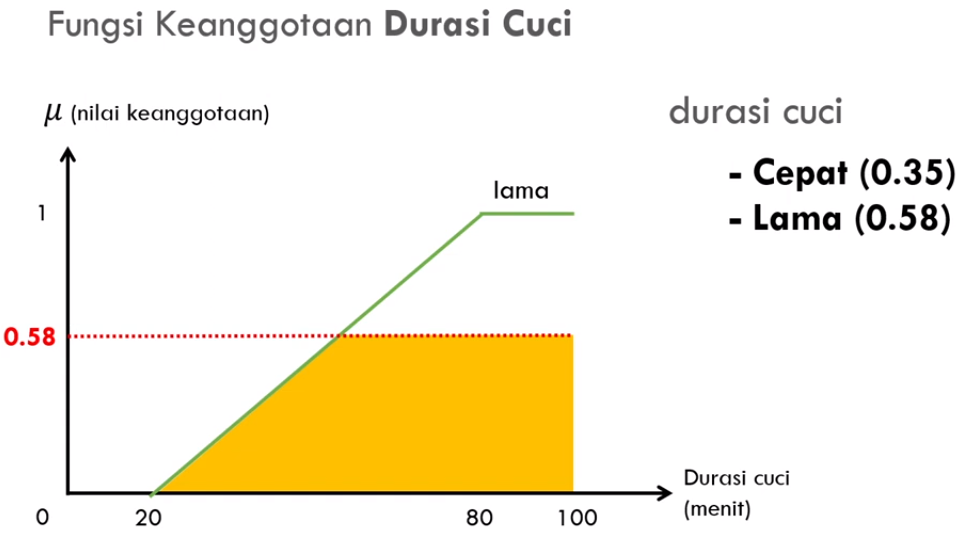
\includegraphics[width=\linewidth]{img/43}
	\end{center}
\end{frame}

\begin{frame}{Defuzification - Mamdani}
	\begin{center}
		\includegraphics[width=\linewidth]{img/44}
	\end{center}
\end{frame}

\begin{frame}{Defuzification - Mamdani}
	\begin{center}
		\includegraphics[width=\linewidth]{img/45}
	\end{center}
\end{frame}

\begin{frame}{Defuzification - Mamdani}
	\begin{center}
		\includegraphics[width=0.8\linewidth]{img/45}
		\includegraphics[width=\linewidth]{img/46}
	\end{center}
\end{frame}

\begin{frame}{Defuzification - Sugeno}
	\begin{center}
		\includegraphics[width=\linewidth]{img/47}
	\end{center}
\end{frame}

\begin{frame}{Perbandingan 3 Metode\\Defuzification}
	\begin{center}
		\includegraphics[width=\linewidth]{img/48}
	\end{center}
\end{frame}

\end{document}
